% !TeX spellcheck = en_GB
%-------------------------------------------------------------------------------
% File: attackTree.tex
%       Vehicle ADVISE project documentation.
%
% Author: Yuri Mazzuoli, Francesco Iemma, Marco Pinna
%         Created on 30/06/2021
%-------------------------------------------------------------------------------
\chapter{Attack tree}\label{ch:attackTree}

\noindent The figure \ref{fig:attackTree} represents the attack tree with the paths that the attackers can follow.

\begin{figure}[H]
    \begin{center}
        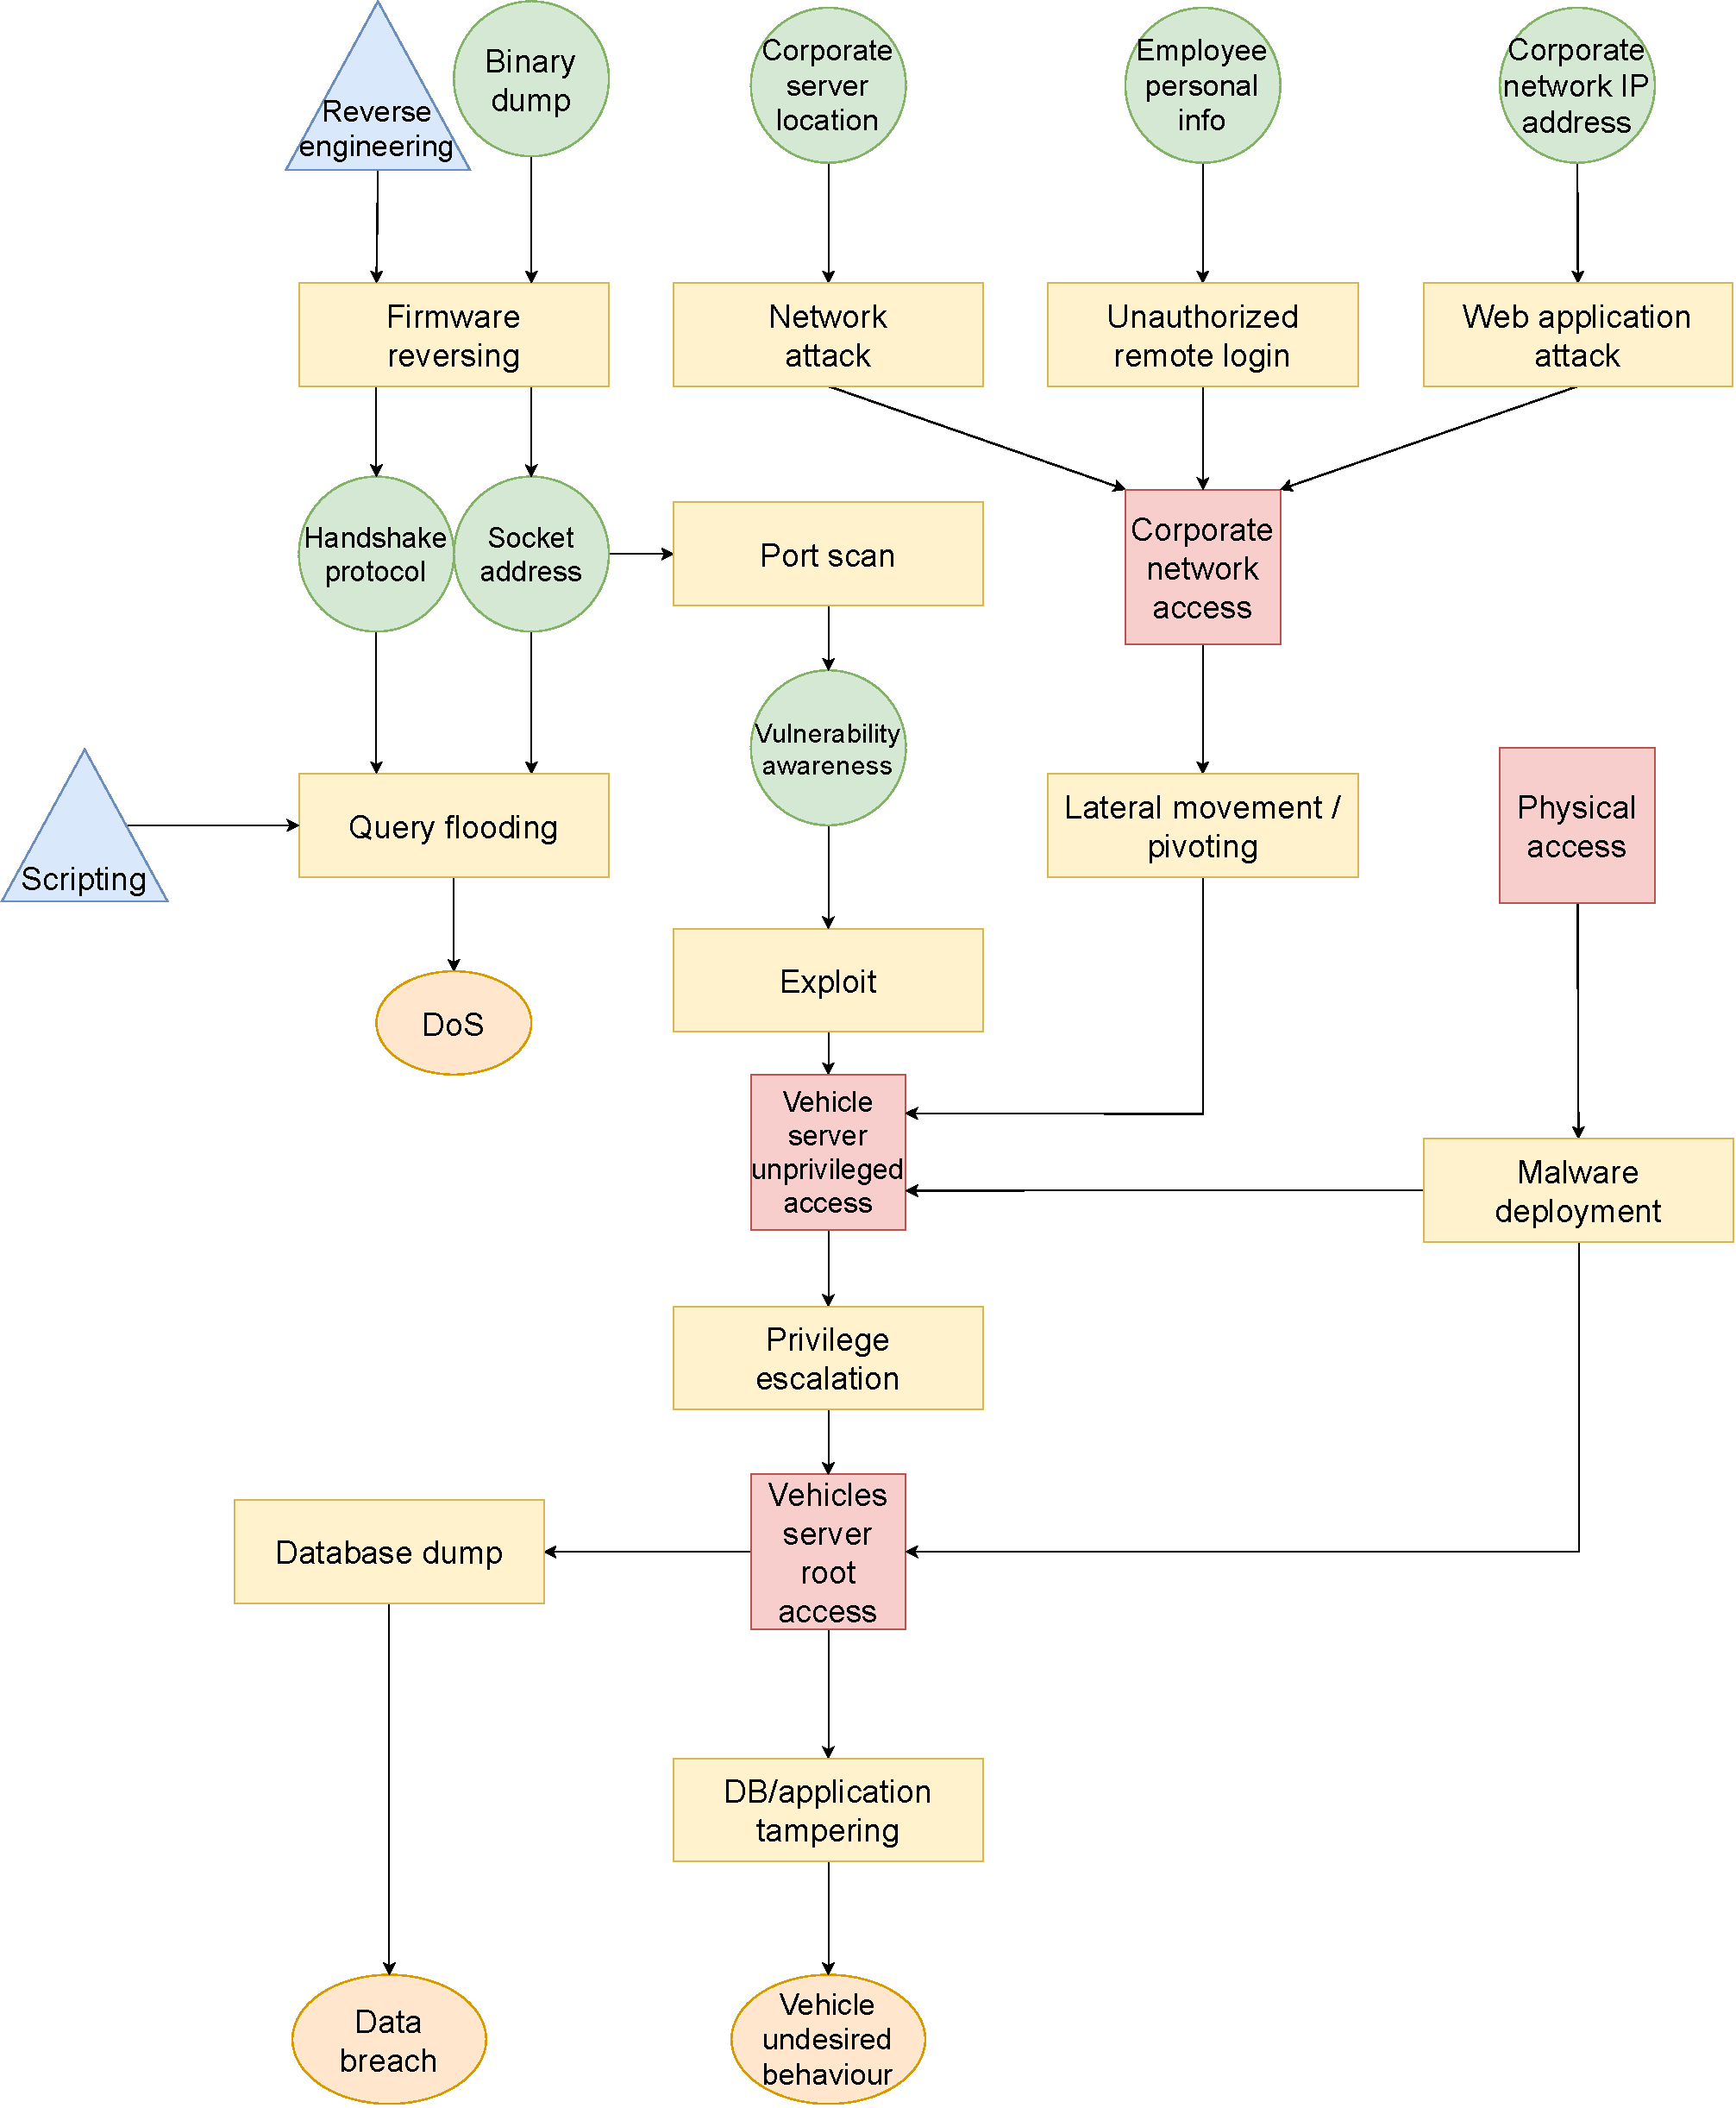
\includegraphics[scale=0.3]{img/attackTree.pdf}
        \caption{Attack tree}
        \label{fig:attackTree}
    \end{center}
    \vspace*{-0.4cm}
\end{figure}

\section{Attacks}
All the attacks has its own probability of achieving results and each of them needs a different time to be executed: in the attack tree we have considered \textit{hours} as unit of time and a deterministic distribution for all the attacks except for the \textit{Query Flooding} (rate equal to 0.1) and \textit{Exploit} (rate equal to 0.2).

\noindent Below there is a brief description of every attack in the tree with the reference to the table used as starting-point (see Appendix A):

\begin{itemize}
	\item \textbf{Firmware reversing}: a hacker in possession of a vehicle and with reverse engineering skills can dump the vehicle firmware, reverse engineer it and acquire information about the IP/port of the server, as well as the protocol used for the communication and/or the structure of the messages sent.
	
	\item \textbf{Query flooding}: a hacker can perform a (D)Dos attack by sending a large number of queries on the server (possibly by means of a botnet) and overwhelming it so that it stops being responsive. (2.1)
	
	\item \textbf{Port scan} with the knowledge of the server's IP, a hacker can scan the server for open ports and possibly find out the OS, which services are running and their versions. 
	
	\item \textbf{Exploit} If an attacker knows a vulnerability inside the system he can exploit it obtaining a root access to the vehicle server. (1.2) 
	
	\item \textbf{Network attack} An insider supposedly already has access to the corporate network but, in case they don't, they can either discover the password in a variety of ways (dictionary attack, password re-use, unattended workstations or laptops) or exploit some vulnerabilities in the Wi-Fi protocol. (1.2)
	
	\item \textbf{Unauthorized remote login}: an attacker could access the corporate VPN by either discovering some employee's login credentials (e.g. phishing, typosquatting, OSINT, social engineering), exploiting some vulnerabilities  in the login procedure itself or by directly having access to credentials (i.e. password dumps found or bought online). (1.2)
	
	\item \textbf{Web application attack}: an attacker could gain unauthorized access to a reserved area of the company's website by means of some web-application attacks (SQLi, XSS, XXE, etc.) or backdoors. (1.2) (3.3)
	
	\item \textbf{Lateral movement/pivoting}: an attacker who has already gained access to a part of the network which is not directly the vehicle server, can exploit further vulnerabilities and ``move laterally" i.e. move deeper inside the network to find more vulnerabilities and entry points that could lead them to the final target server. (1.1) (1.2) (3.1) (3.3)
	
	\item \textbf{Malware deployment}: an attacker can deploy a malware in different ways e.g. dropping an infected USB drive and wait for some employee to plug it in a corporate machine. The malware can guarantee them the access to a server with a varying level of privilege. (1.3) (3.4)
	
	\item \textbf{Privilege escalation}: once an attacker has gained the so-called ``foothold" into the target server, they will try to increase their privilege level on the system as to access to a greater number of resources. (1.2) (3.4)	
	
	\item \textbf{Database dump}: once the attacker has gained access to the database, the latter can be dumped and the \textit{Data Breach} goal is reached. For the sake of simplicity the \texttt{database dump} attack in the tree is considered to have constant time duration and probability of detection. In reality this is not the case as there are different ways to perform data exfiltration, which can be more or less stealthy (simple \texttt{scp} or \texttt{wget} commands -- or their equivalent on non-Unix systems -- will be faster but they will also have a high probability of detection while looking at the network traffic and the server logs, while other techniques such as ICMP exfiltration will be stealthier at the expense of a longer time required). (3.2) (3.5)
	
	\item \textbf{DB/application tampering}: if the goal of the attacker is not to access sensitive data but to cause undesired behaviour of the vehicles, once they have access to the DB or the application they can tamper the data in the DB, or attack the application/framework that is running on the server and which interacts with the vehicles. (2.1) (3.2)
\end{itemize}